%%%%%%%%%%%%%%%%%%%%%%%%%%%%%%%%%%%%%%%%%
% Journal Article
% LaTeX Template
% Version 1.3 (9/9/13)
%
% This template has been downloaded from:
% http://www.LaTeXTemplates.com
%
% Original author:
% Frits Wenneker (http://www.howtotex.com)
%
% License:
% CC BY-NC-SA 3.0 (http://creativecommons.org/licenses/by-nc-sa/3.0/)
%
%%%%%%%%%%%%%%%%%%%%%%%%%%%%%%%%%%%%%%%%%

%----------------------------------------------------------------------------------------
%	PACKAGES AND OTHER DOCUMENT CONFIGURATIONS
%----------------------------------------------------------------------------------------

\documentclass[twoside]{article}

\usepackage{lipsum} % Package to generate dummy text throughout this template

\usepackage[sc]{mathpazo} % Use the Palatino font
\usepackage[T1]{fontenc} % Use 8-bit encoding that has 256 glyphs
\linespread{1.05} % Line spacing - Palatino needs more space between lines
\usepackage{microtype} % Slightly tweak font spacing for aesthetics

\usepackage[hmarginratio=1:1,top=32mm,columnsep=20pt]{geometry} % Document margins
\usepackage{multicol} % Used for the two-column layout of the document
\usepackage[hang,small,labelfont=bf,up,textfont=it,up]{caption} % Custom captions under/above floats in tables or figures
\usepackage{booktabs} % Horizontal rules in tables
\usepackage{float} % Required for tables and figures in the multi-column environment - they need to be placed in specific locations with the [H] (e.g. \begin{table}[H])
\usepackage{hyperref} % For hyperlinks in the PDF

\usepackage{lettrine} % The lettrine is the first enlarged letter at the beginning of the text
\usepackage{paralist} % Used for the compactitem environment which makes bullet points with less space between them
\usepackage{graphicx} % Used for including images

\usepackage{abstract} % Allows abstract customization
\renewcommand{\abstractnamefont}{\normalfont\bfseries} % Set the "Abstract" text to bold
\renewcommand{\abstracttextfont}{\normalfont\small\itshape} % Set the abstract itself to small italic text

\usepackage{titlesec} % Allows customization of titles
\renewcommand\thesection{\Roman{section}} % Roman numerals for the sections
\renewcommand\thesubsection{\Roman{subsection}} % Roman numerals for subsections
\titleformat{\section}[block]{\large\scshape\centering}{\thesection.}{1em}{} % Change the look of the section titles
\titleformat{\subsection}[block]{\large}{\thesubsection.}{1em}{} % Change the look of the section titles

\usepackage{fancyhdr} % Headers and footers
\pagestyle{fancy} % All pages have headers and footers
\fancyhead{} % Blank out the default header
\fancyfoot{} % Blank out the default footer
\fancyhead[C]{Boulder Flood Impacts Pre-flood and Post-flood - 2013 $\bullet$ March 2015 $\bullet$ No. 1} % Custom header text
\fancyfoot[RO,LE]{\thepage} % Custom footer text

%----------------------------------------------------------------------------------------
%	TITLE SECTION
%----------------------------------------------------------------------------------------

\title{\vspace{-15mm}\fontsize{24pt}{10pt}\selectfont\textbf{Boulder Flood Impacts Pre-flood and Post-flood - 2013}} % Article title

\author{
\large
\textsc{John Raesly}\thanks{A thank you or further information}\\[2mm] % Your name
\normalsize University of Colorado - Boulder \\ % Your institution
\normalsize \href{mailto:john.raesly@gmail.com}{john.raesly@gmail.com} % Your email address
\vspace{-3mm}
}
\date{3/29/2015}

%----------------------------------------------------------------------------------------

\begin{document}

\maketitle % Insert title

\thispagestyle{fancy} % All pages have headers and footers

%----------------------------------------------------------------------------------------
%	ABSTRACT
%----------------------------------------------------------------------------------------

\begin{abstract}

The 2013 flood in Boulder, called the 100 year flood, was a natural disaster for the century. The floods power changed much of the ecosystem that surrounds Boulder, CO. The purpose of this project is to examine the 2013 flood in Boulder, CO and its impacts on the river morphology of the creeks and rivers surrounding Boulder, CO and the change in land cover that occurred. Direct correlations between the rivers the amount of rainfall in those areas feeding into the rivers are of interest. In particular, this study will investigate: How river morphology has changed from pre to post flood?; Do areas designated as floodplains affect the river change?; What is the correlation between rainfall amounts and river density change?; What is the land cover compared to water cover for pre versus post flood? QGIS will be utilized to convert the files to shapefiles (.shp) and other usable formats for GRASS GIS. Then Grass GIS will be used to integrate an analysis method for the raster data and dissolve it as necessary. Previous techniques from other flood studies that have shown to be effective will be analyzed. Sources will include the Boulder Open GIS, which has some from the NOAA Disaster Data to analyze similar conditions (rainfall amount). This study will focus on Boulder County in Colorado. 

\end{abstract}

%----------------------------------------------------------------------------------------
%	ARTICLE CONTENTS
%----------------------------------------------------------------------------------------

\begin{multicols}{2} % Two-column layout throughout the main article text

\section{Introduction}

\lettrine[nindent=0em,lines=3]{U}nderstanding the river morphology for the Boulder 2013 Flood is important for assesing the floodplains that are at the top concern if such an event were to happen again. The 2013 flood in Boulder was a natural disaster that could be cause for concern. The flood changed the stream channel within Boulder County, CO. This study focuses specifically on Boulder County. In this study, the 2013 flood in Boulder, CO is examined and its impacts on the river morphology of the creeks and rivers surrounding Boulder, CO and the change in land cover that occurred. Direct correlations between the rivers the amount of rainfall in those areas feeding into the rivers are of interest. In particular, this study will investigate: How river morphology has changed from pre to post flood?; Do areas designated as floodplains affect the river change?; What is the correlation between rainfall amounts and river density change?; What is the land cover compared to water cover for pre versus post flood? Established are concrete ways for examining the questions at hand.
%------------------------------------------------

\section{Methods}

\begin{figure*} % figure* spans two columns, figure is just one column
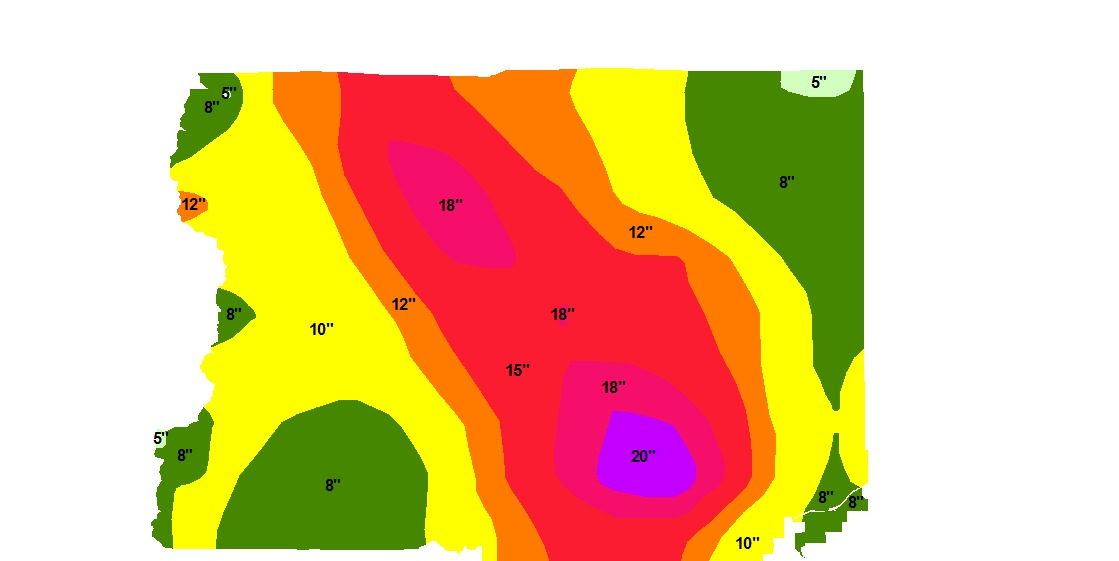
\includegraphics[width=2\columnwidth]{project.jpg}
\caption{Rainfall Distribution\label{fig:sloth}}
\end{figure*}

Developed were several measures to assess the stream channel - pre flood against the stream channel - post flood shapefiles.
\begin{compactitem}
\item Clip the shapefiles
\item Find the difference in the shapefiles
\item Branch shapefiles and find flow patterns
\item Assign rainfall minimum and maximum attribute for Boulder County
\item Assign generall rainfall minimum and maximum to separated areas
\item Correlate the rainfall amounts against the post-flood stream channel
\end{compactitem}
\subsection{Clip the Shapefiles}
Qgis was used for most operations during this research. Using the built-in function, Clip, was able to show the the similarities in both of the shapefiles. It created a new shape based on the area of the input layer that is overlapped by the clipping layer. The attributes of the chosen layer only were copied to the new feature With the new information of which parts stayed the same, it was then useful to examine the portion that did not change. It was then discovered that only a small portion of the stream channel did not change. In figure 1(image file not created yet), you can view the similar stream channel across Boulder County.

\begin{figure*} % figure* spans two columns, figure is just one column
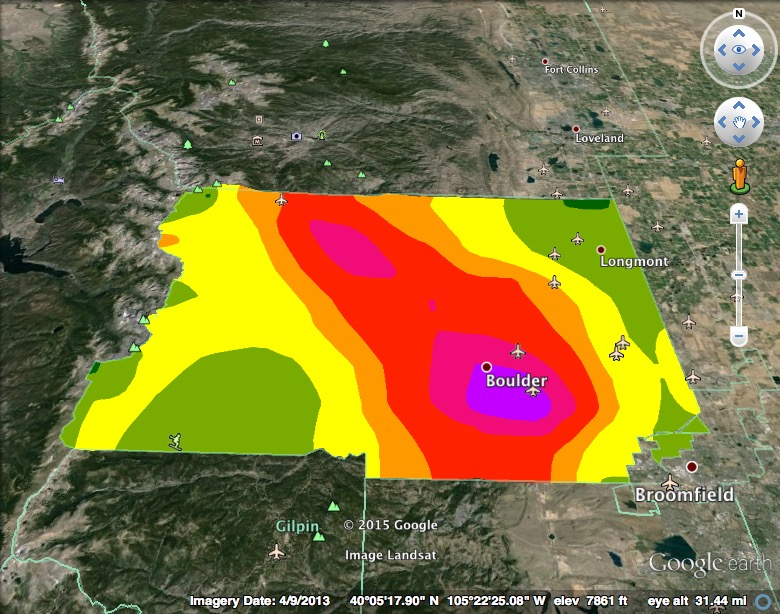
\includegraphics[width=2\columnwidth]{earth.jpg}
\caption{Rainfall Distribution over Boulder County\label{fig:earth}}
\end{figure*}

\subsection{Find the Difference in Shapefiles}
The difference function in Qgis was then used to determine the difference in the two shapefiles being examined. Both of the shapefiles had the same attributes which made it simpler to compare and contrast. The difference function created a new feature based on the area of the input layer that was not overlapped by the clipping layer.



\subsection{Assign Rainfall Attribute for Boulder County}
The purpose of this part was to assign a general legend for each area that fell into similar rainfall mininum and maximum ranges. The numbers can be viewed in figure 1. It was based upon finding a general rule for each set of values for the designated areas. 
%\begin{table}[H]
%\caption{Rainfall Attribute Table}
%\centering
%\begin{tabular}{llr}
%\toprule
%\multicolumn{2}{c}{Name} \\
%\cmidrule(r){1-2}
%First name & Last Name & Grade \\
%\midrule
%John & Doe & $7.5$ \\
%Richard & Miles & $2$ \\
%\bottomrule
%\end{tabular}
%\end{table}


\subsection{Correlate Rainfall and Post-flood River Morphology}
The correlation was created by implementing Spatial Autocorrelation within Qgis. It was also easily viewed by overlapping the rainfall data with the post-flood stream channel shapefile. Which can be viewed at figure 4. 
\begin{figure*} % figure* spans two columns, figure is just one column
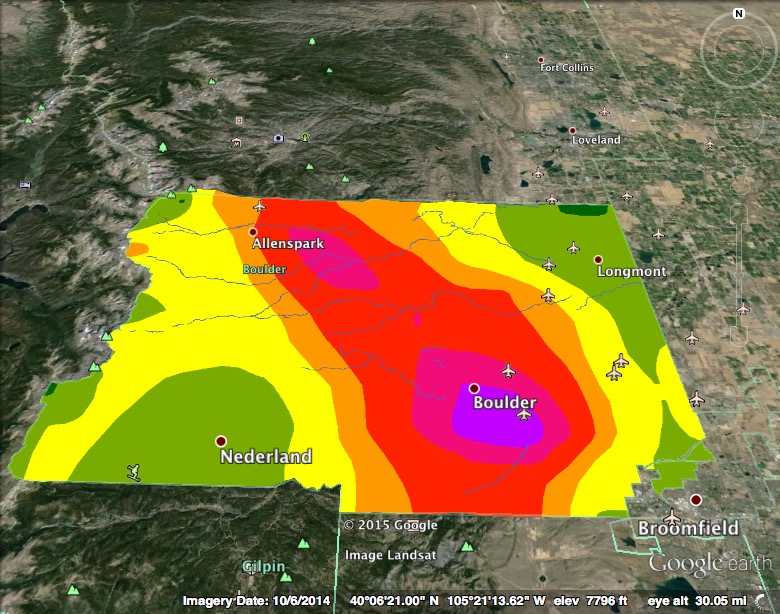
\includegraphics[width=1.6\columnwidth]{preflood.jpg}
\caption{Pre-Flood Stream Channel and Rainfall Distribution\label{fig:preflood}}
\end{figure*}
\begin{figure*} % figure* spans two columns, figure is just one column
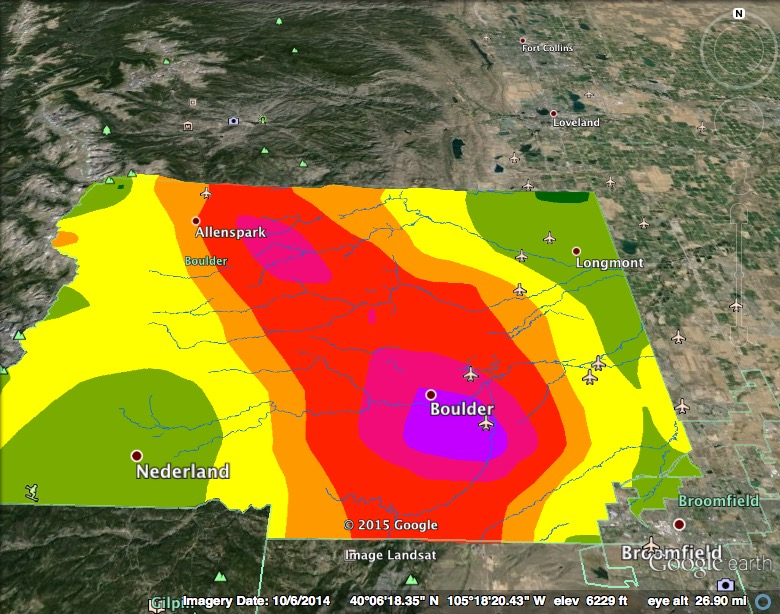
\includegraphics[width=1.6\columnwidth]{postflood.jpg}
\caption{Post-Flood Stream Channel and Rainfall Distribution\label{fig:postflood}}
\end{figure*}

%------------------------------------------------

\section{Results}

%\begin{table}[H]
%\caption{Example table}
%\centering
%\begin{tabular}{llr}
%\toprule
%\multicolumn{2}{c}{Name} \\
%\cmidrule(r){1-2}
%First name & Last Name & Grade \\
%\midrule
%John & Doe & $7.5$ \\
%Richard & Miles & $2$ \\
%\bottomrule
%\end{tabular}
%\end{table}

About (put percent here) of the stream channel stayed consistent with the pre-flood stream channel during this disaster. The mass of the findings concluded that most of the now stream channel was newly created. The post-flood stream channel is mostly represented by the rainfall that happened during the flood. Where there was less rain, most of those channels have dissapeared and dispersed into the areas where there was the most rainfall. There was very little stream channel in Boulder, CO pre-flood, but now there are many new streams that have been created because of this flood and it mostly amounts to the mass rainfall that was recorded in the Southwestern part of the county. 

%\begin{equation}
%\label{eq:emc}
%e = mc^2
%\end{equation}


%------------------------------------------------

\section{Discussion}

The entirety of this disaster created many new stream channels throughout Boulder County. Whereas most of the stream channel occured in the Northwestern part of the county it is now distributed evenly throughout the county with more of it leaning towards the eastern border. Large amounts of rainfall can be extremely effective in rerouting a whole river system. This causes many unknown side effects. There could be a loss of habitat in the area that for so long had relied on the river system, but the newly created streams could thrive and welcome all new sorts of habitat. This does mess up the ecological balance that nature depends on. It is like taking the wolves out of Yellowstone. We will not know the seriousness of these changes until many years later, which is something that should be investigated. As there are now many reasons to attribute to habitat loss, ie global warming, the main focus should be upon the species that whole heartedly relied upon the previous river system. Another focus of study should be if there are new disasters that were previously averted because of the river morphology. One of the disasters could be the snow melt and the floodplains. Does the new stream channel cause concern for residents situated around these floodplains that were previously unaffected?


%----------------------------------------------------------------------------------------

\end{multicols}

\end{document}
